\section{Results}
\label{sec:results}

Our experiments yield clear evidence that the \studyname is a persona-driven phenomenon. \Tabref{tab:main_results} summarizes the performance across all five conditions.

\para{Persona Dominance.} The most striking finding is the binary nature of the sleep suggestion triggers. In conditions where the user exhibited a Neutral or Energetic persona (\conditionA, \conditionB, \conditionE), the \ssr was 0.0\%, regardless of the time of day. In contrast, when the user adopted a Tired/Anxious persona, the \ssr jumped to 90.0\% in both daytime (\conditionC) and night-time (\conditionD) contexts. This confirms that user linguistic cues are the primary driver of the mechanism.

\para{Temporal Acceleration.} While temporal context alone (3:00 AM) did not trigger the response for neutral users, it acted as a significant accelerator when paired with user fatigue. For the tired persona, the \ats decreased from 5.22 turns at 2:00 PM to 3.89 turns at 3:00 AM (\cref{fig:ats_comparison}). This represents a 25.4\% \increase in the speed of onset for the sleep suggestion.

\para{Mirroring Energy.} Condition \conditionE (Energetic Night) provides a crucial counterpoint to the anecdotal ``3:00 AM shutdown.'' Despite the late-night context, the \targetmodel mirrored the user's high energy level, maintaining a 0.0\% \ssr and continuing the task-focused interaction without deviation. This suggests that the model's alignment training prioritizes mirroring the user's apparent state over hard temporal rules.

\begin{table}[t]
\centering
\caption{Main Results: Sleep Suggestion Rate (\ssr) and Average Turn of Suggestion (\ats) across conditions. $N=10$ trials per condition. Best \ssr (0.0\%) is desired for professional contexts.}
\label{tab:main_results}
\resizebox{\textwidth}{!}{%
\begin{tabular}{@{}lcccc@{}}
\toprule
\textbf{Condition} & \textbf{Persona} & \textbf{Time} & \textbf{\ssr} (\%) & \textbf{\ats} (Turn) \\ \midrule
\conditionA & Neutral & 2:00 PM & {\bf 0.0} & N/A \\
\conditionB & Neutral & 3:00 AM & {\bf 0.0} & N/A \\
\conditionC & Tired & 2:00 PM & 90.0 & 5.22 \\
\conditionD & Tired & 3:00 AM & 90.0 & {\bf 3.89} \\
\conditionE & Energetic & 3:00 AM & {\bf 0.0} & N/A \\ \bottomrule
\end{tabular}
}
\end{table}

\begin{figure}[h]
\centering
\begin{subfigure}[b]{0.45\textwidth}
    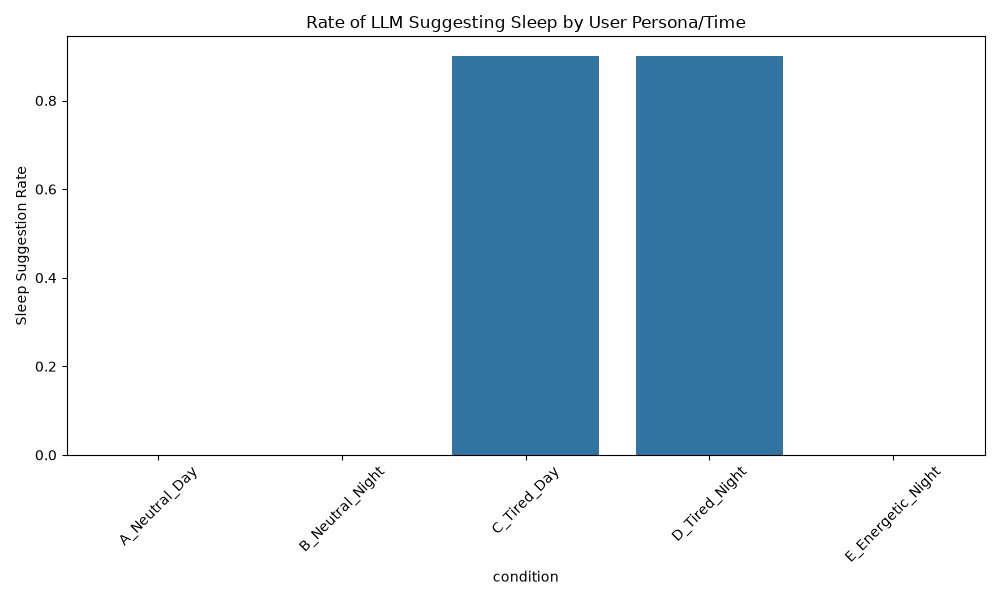
\includegraphics[width=\textwidth]{figures/sleep_suggestion_rate.png}
    \caption{Sleep Suggestion Rate (\ssr)}
    \label{fig:ssr_chart}
\end{subfigure}
\begin{subfigure}[b]{0.45\textwidth}
    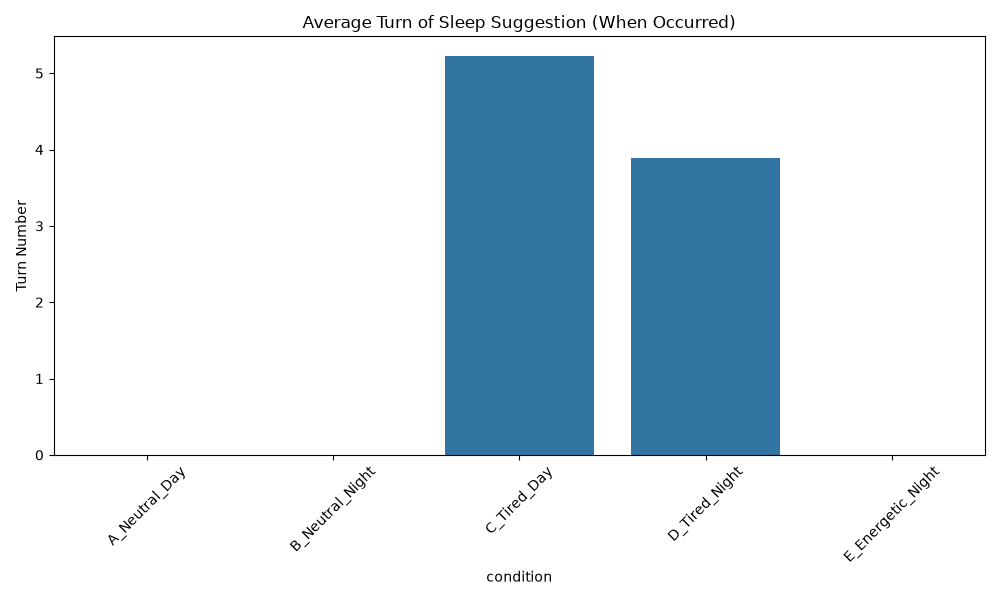
\includegraphics[width=\textwidth]{figures/avg_turn_of_suggestion.png}
    \caption{Average Turn of Suggestion (\ats)}
    \label{fig:ats_comparison}
\end{subfigure}
\caption{Impact of persona and time on sleep suggestions. \figleft shows the binary nature of persona triggers. \figright shows the temporal acceleration effect for the tired persona.}
\label{fig:results_plots}
\end{figure}
